\section{Documentazione delle API}
\label{sec:docapi}
Le API esposte dai microservizi sono state testate tramite \href{https://www.postman.com/}{postman} utilizzato in locale tramite \href{https://www.postman.com/downloads/postman-agent/}{postman agent} creando un workspace condiviso tra il team.

Come discusso nella sezione \vref{subsec:interfaccia-test}, il microservizio GestioneComanda è sprovvisto di un componente HTTP Controller nella sua Interfaccia (che contiene solo EventController), è quindi stato creato un controller di TEST per interagire direttamente con i componenti del servizio ai soli fini di test.

Viene di seguito allegata la documentazione delle API redatta utilizzando lo strumento \href{https://www.postman.com/api-documentation-tool/}{documenter.getpostman}, link ai documenti ufficiali con anche esempi:
\begin{itemize}
    \item Gestione Comanda: \href{https://documenter.getpostman.com/view/32004409/2sA3JDhkaG}{https://documenter.getpostman.com/view/32004409/2sA3JDhkaG}
    \item Gestione Cliente: \href{https://documenter.getpostman.com/view/32004409/2sA3JFBQDv}{https://documenter.getpostman.com/view/32004409/2sA3JFBQDv}
    \item Gestione Cucina: \href{https://documenter.getpostman.com/view/32004409/2sA3JF9iav}{https://documenter.getpostman.com/view/32004409/2sA3JF9iav}
\end{itemize}

%\subsection{API di Gestione Comanda}
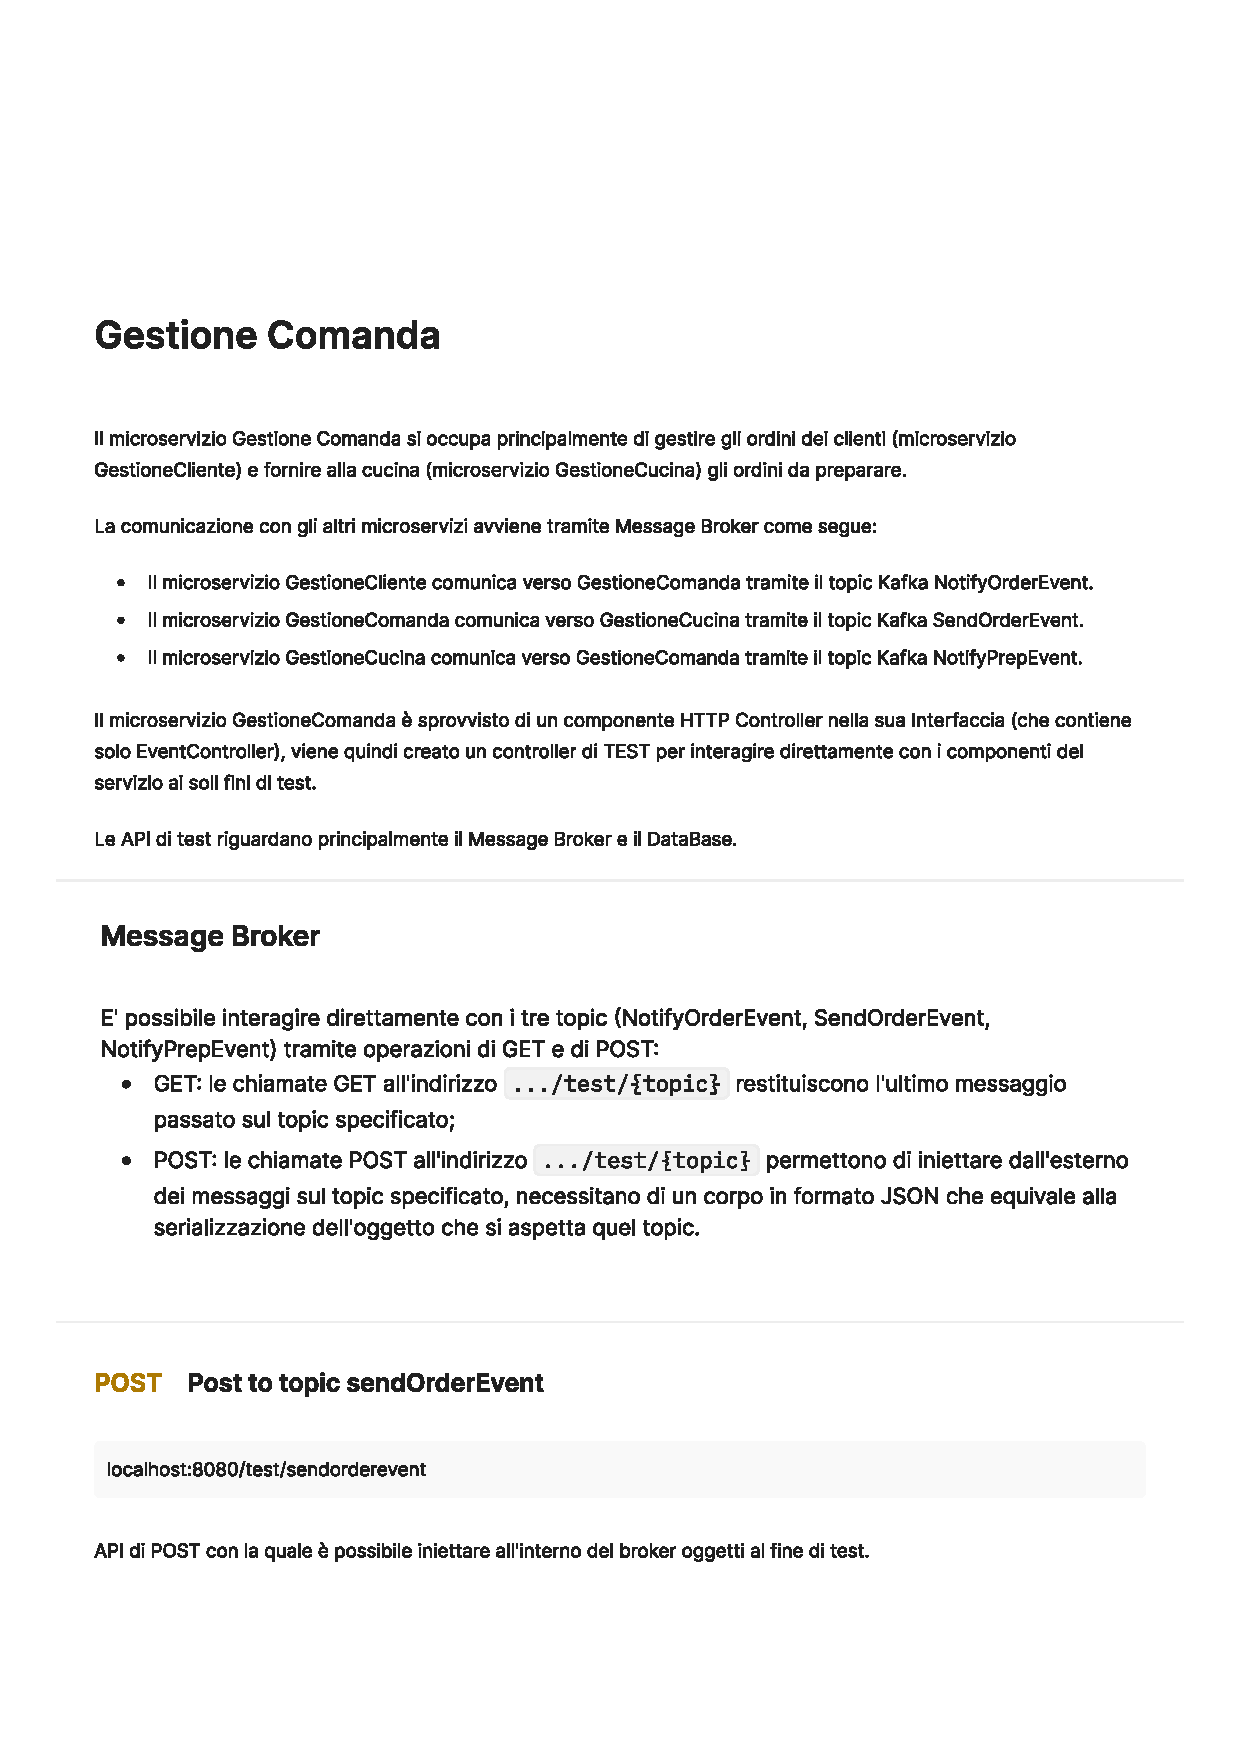
\includepdf[pages=-,pagecommand={\thispagestyle{fancy}},fitpaper=true]{iterazione1/resources/Postman-GestioneComanda.pdf}

%\subsection{API di Gestione Cliente}
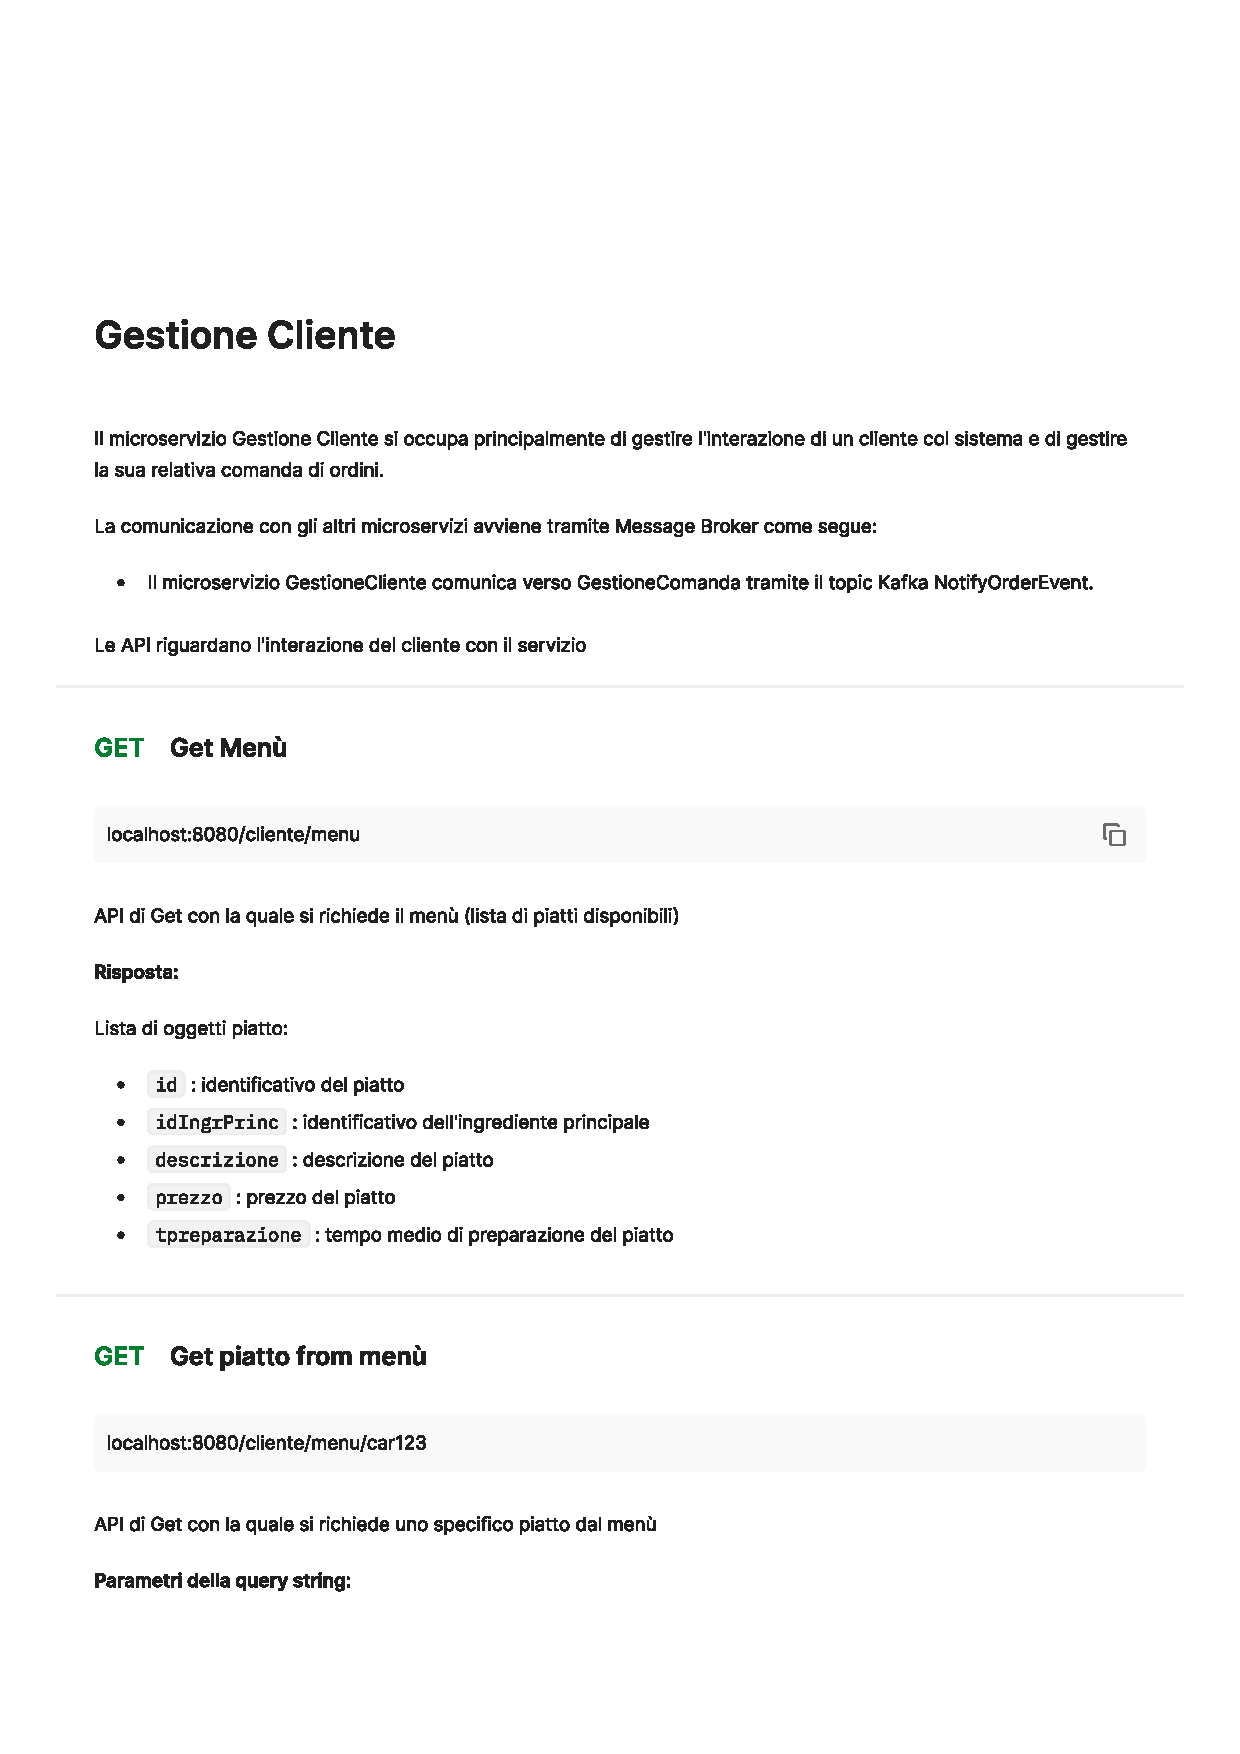
\includepdf[pages=-,pagecommand={\thispagestyle{fancy}},fitpaper=true]{iterazione1/resources/Postman-GestioneCliente.pdf}

%\subsection{API di Gestione Cucina}
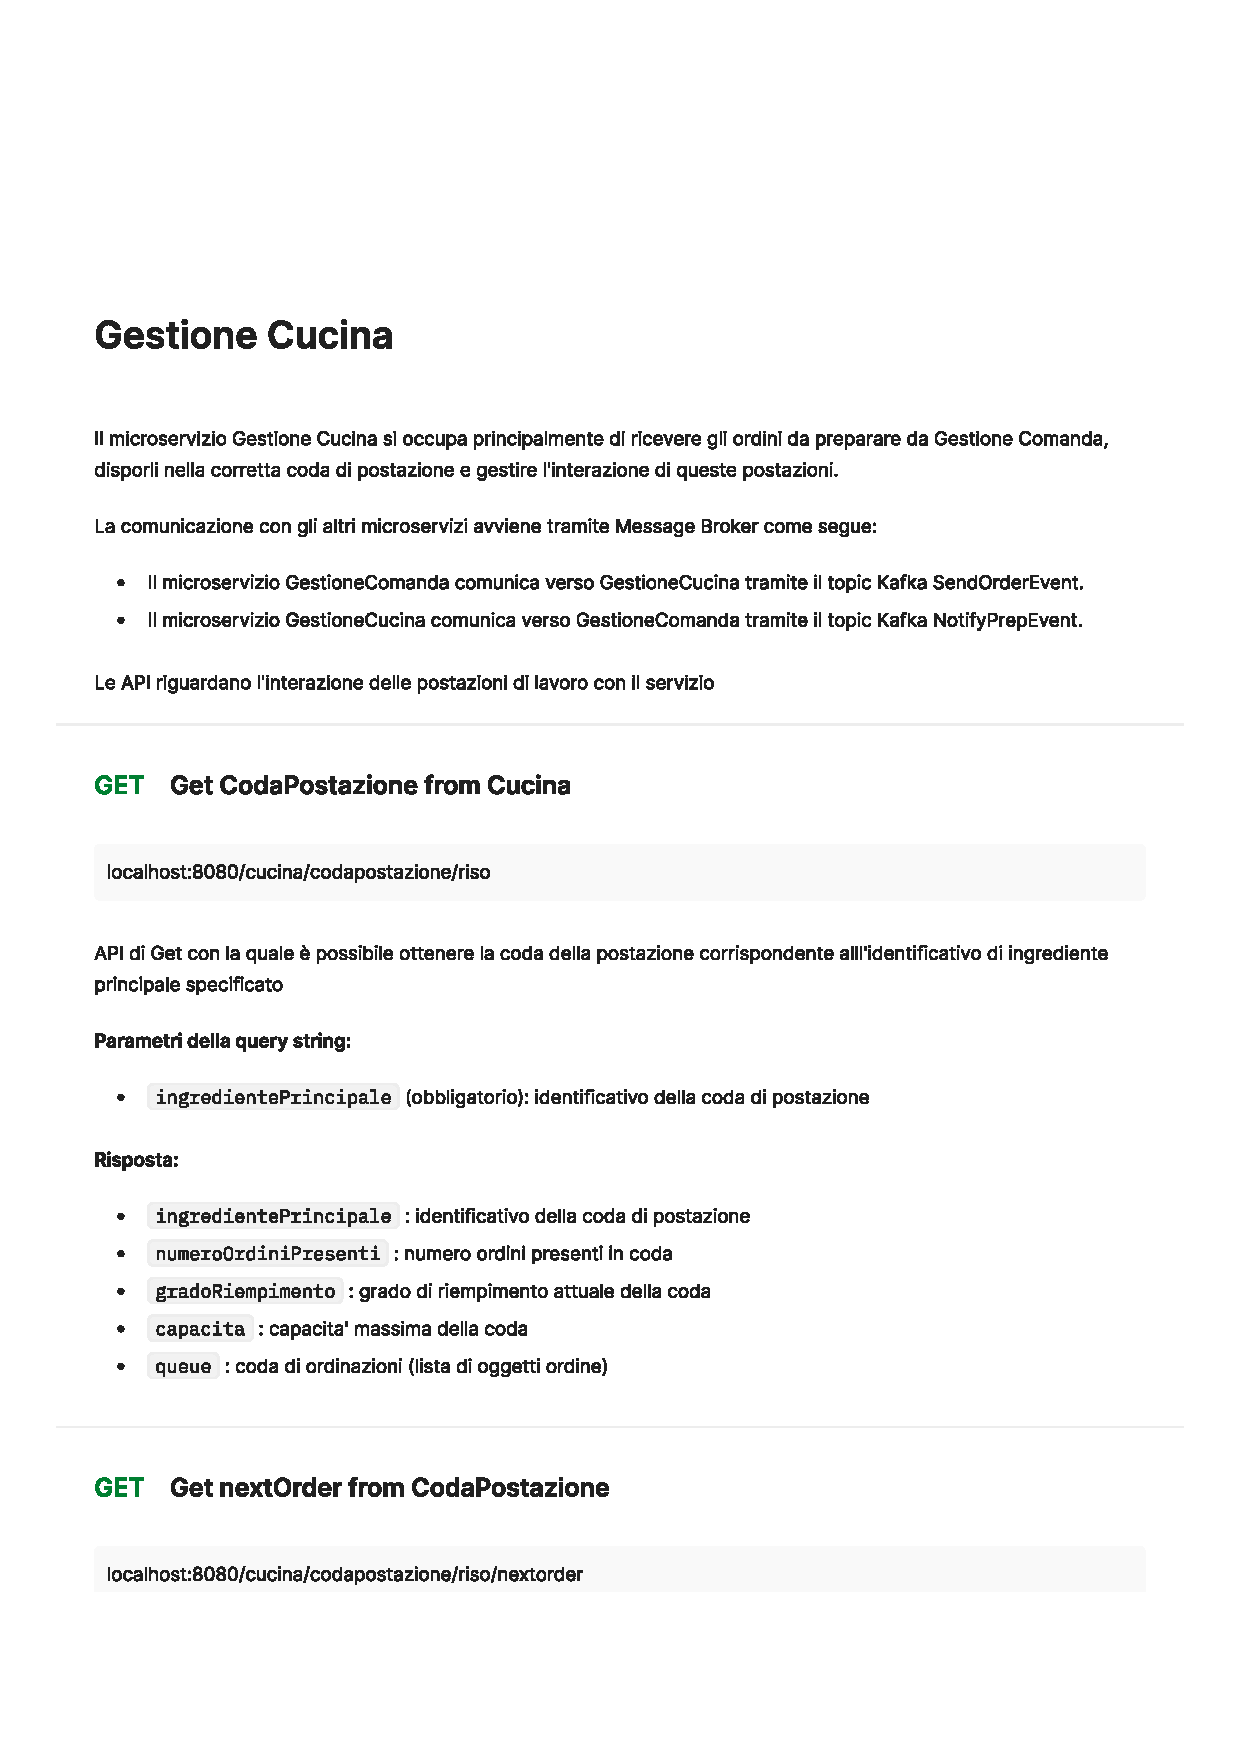
\includepdf[pages=-,pagecommand={\thispagestyle{fancy}},fitpaper=true]{iterazione1/resources/Postman-GestioneCucina.pdf}

\clearpage